% !TeX program = lualatex
% !TeX root = luaking.tex
% !TeX encoding = UTF-8
% !TeX spellcheck = cs_CZ
%=========================== Kapitola: Zákony termodynamiky =======================================
\setchaptertoc
\chapter{Zákony termodynamiky}\label{fyz:IchapXLIV}

  \section{Tepelné stroje; první zákon}\label{fyz:IchapXLIVsecI}
    Dosud jsme mluvili o vlastnostech hmoty z atomového hlediska a snažili jsme se aspoň zhruba
    pochopit, co se bude dít, předpokládáme-li, že hmota se skládá z atomů podléhajících určitým
    zákonům. Existuje však mnoho vztahů mezi vlastnostmi látek, k nimž můžeme dospět bez podrobné
    znalosti jejich struktury. Určování vztahů mezi různými vlastnostmi látek, bez poznání jejich
    vnitřní struktury je předmětem \textbf{termodynamiky}. Termodynamika vznikla dříve, než byla
    známa vnitřní struktura hmoty.
    
    Uveďme příklad: Z kinetické teorie víme, že tlak plynu je způsobován nárazy molekul a víme i to,
    že když plyn zahřejeme, nárazy molekul zesílí, a proto musí tlak vzrůst. Naopak, pohybuje-li se
    píst v nádobě s plynem proti síle těchto nárazů, energie molekul narážejících na píst vzroste, a
    proto vzroste i teplota. Zvýšíme-li tedy při daném objemu teplotu, zvýšíme tlak. Na druhé
    straně, stlačíme-li plyn, zjistíme, že jeho teplota vzrostla. Z kinetické teorie můžeme odvodit
    kvantitativní vztah mezi těmito dvěma jevy, ale instinktivně tušíme, že mezi nimi musí existovat
    nějaká souvislost, která nezávisí na konkrétním průběhu srážek. 
    
    Všimněme si jiného příkladu - zajímavé vlastnost gumy: Když roztáhneme pásek gumy, zahřeje se.
    Vložíme-li si takový pásek mezi rty a natáhneme ho, pocítíme, že se zahřál a toto zahřátí je
    vratné v tom smyslu, že při rychlém uvolnění pásku pocítíme na rtech ochlazení. To znamená, že
    při napínání pásek gumy hřeje a při uvolňování pásek chladí. Náš instinkt nám napoví, že zahřátá
    guma může tahat: skutečnost, že při napnutí se pásek zahřál, nás přivede k závěru, že zahřátí
    pásku vyvolá jeho smrštění. A skutečně, ohřejeme-li plynovým kahanem pásek gumy držící závaží,
    zpozorujeme, že se pásek náhle stáhl (obr. \ref{fyz:fig467}). Je tedy pravda, že při zahřívání
    se guma smršťuje a tato skutečnost je ve shodě s tím, že při uvolňování jejího napětí guma
    chladne.

    \begin{figure}[ht!] %\ref{fyz:fig467}
      \centering
      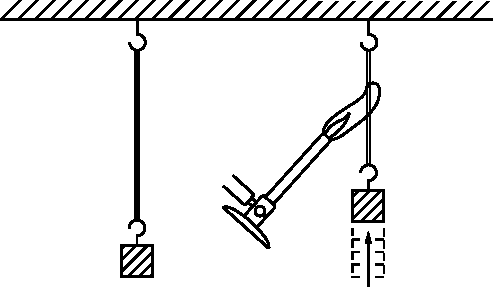
\includegraphics[width=0.7\linewidth]{fyz_fig467.pdf}
      \caption{ Zahřátý pásek gumy (\cite[s.~596]{Feynman01})}
      \label{fyz:fig467}
    \end{figure}

    Vnitřní mechanizmus gumy způsobující tyto jevy je velmi složitý. Popíšeme ho do určité míry z
    molekulového hlediska, i když hlavním cílem této kapitoly je pochopit vztahy mezi takovými jevy
    nezávisle na molekulovém modelu. Na základě molekulového modelu můžeme ukázat, že tyto jevy úzce
    souvisí. Jeden ze způsobů, jak můžeme pochopit chování gumy, spočívá v představě, že guma se
    skládá z ohromného svazku dlouhých molekulových řetězců, jakýchsi „molekulových špaget“ s
    jednou dodatečnou komplikací: řetězce jsou vzájemně propojeny - jakoby se některé křížem
    procházející špagety svařily a vytvořily tak velké klubko. Natahujeme-li takové klubko, některé
    z řetězců se snaží seřadit do směru tahu. Řetězce jsou zároveň v tepelném pohybu a neustále do
    sebe narážejí. Řetězec nezůstane sám od sebe natažen, neboť ze stran do něho narážejí jiné
    řetězce a jiné molekuly a přinutí ho opět se stáhnout. Skutečná příčina toho, že gumový pásek se
    snaží smrštit, spočívá v následujícím: když ho natáhneme, řetězce se prodlouží, ale tepelné
    působení molekul ze stran se snaží řetězce zkroutit, a tak je zkrátit. K příznivé situaci
    dochází tehdy, když jsou řetězce napnuty  a zvýšíme teplotu; tehdy zesílí i bombardování řetězců
    ze stran, řetězce mají snahu se stáhnout a jsou proto při zahřátí schopny zdvihnout těžší
    závaží. Dovolíme-li pásku gumy po určitém čase napnutí se uvolnit, stane se každý řetězec měkčím
    a molekuly narážející do uvolněných řetězců ztrácejí energii. Proto teplota klesá.

    Viděli jsme, jak kinetická teorie uvádí do souvislosti tyto dva procesy, smrštění při zahřívání
    a ochlazení během uvolňování, ale bylo by úžasně složité určit přesný vztah mezi nimi z teorie.
    Museli bychom znát počet srážek za sekundu a tvar řetězců a vzít v úvahu všechny možné
    komplikace. Podrobnosti mechanizmu jsou tak složité, že pomocí kinetické teorie opravdu
    nemůžeme přesně určit, co se odehrává; můžeme však odvodit určité vztahy mezi těmito
    pozorovanými jevy aniž bychom něco věděli o vnitřním mechanizmu.

    Celá termodynamika spočívá na úvahách následujícího druhu: protože pásek gumy je při vysokých
    teplotách „silnější“ než při nízkých, mělo by být možné zdvíhat závaží a přemisťovat je a konat
    tak práci pomocí tepla. Už jsme se vlastně experimentálně přesvědčili, že zahřátý pásek gumy
    může zdvíhat závaží. \emph{Rozvoj termodynarniky začal studiem toho, jak můžeme pomocí tepla
    konat práci.} Můžeme sestrojit zařízení, jež by ke konání práce využívalo vliv tepla na gumový
    pásek? Ano, takové zařízení můžeme sestrojit, i když bude vypadat hloupě. Skládá se z kola
    bicyklu, které má místo drátů gumové pásky (obr. \ref{fyz:fig468}). Zahříváme-li gumové pásky na
    jedné straně kola dvojicí výhřevných lamp, stanou se „silnější“ než gumové pásky na druhé straně
    kola. Těžiště kola se posune na stranu, mimo ložisko, a kolo se pootočí. Tak se chladné gumové
    pásky dostanou k teplu, teplé se vzdálí a ochladí a kolo se bude pomalu otáčet, dokud budou
    lampy hřát.

    \begin{figure}[ht!] %\ref{fyz:fig468}
      \centering
      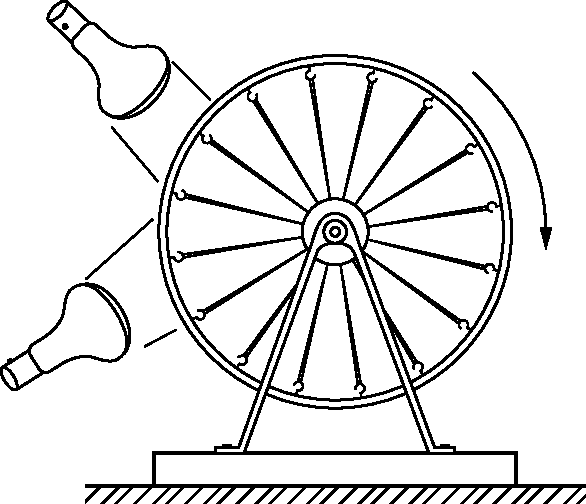
\includegraphics[width=0.7\linewidth]{fyz_fig468.pdf}
      \caption{ Tepelný stroj s pásky gumy (\cite[s.~707]{Feynman01})}
      \label{fyz:fig468}
    \end{figure}

    Účinnost takového stroje je mimořádně nízká. Výkon 400 wattů potřebný k ohřívání lamp stačí
    právě tak na zdvihnutí mouchy! Nabízí se proto zajímavá otázka, zda teplo může konat práci s
    podstatně vyšší účinností.

    Zrod termodynamiky se vlastně váže na analýzu slavného inženýra Sadi Carnota, kterého zaujal
    problém konstrukce nejlepšího a nejúčinnějšího stroje. Byl to jeden z mála pozoruhodných
    případů, kdy technika přispěla podstatným způsobem k fyzikální teorii. Jiným případem, je
    analýza informační teorie podaná Claudem Shannonem. Mimochodem, tyto problémy spolu úzce
    souvisí.

    Parní stroj pracuje obvykle tak, že teplo ohně uvádí do varu vodu, a takto vytvořená pára se
    rozpíná, tlačí na píst a ten uvádí do chodu kolo. Takže pára zatlačí píst - a co potom s ní?
    Načatou činnost je třeba dokončit a bylo by hloupé skončit cyklus tím, že necháme páru
    uniknout do vzduchu, vždyť bychom museli stále dodávat vodu. Je levnější - účinnější - nechat
    proudit páru do jiné nádrže, kde ji zkondenzujeme studenou vodou a pak ji opět přečerpáme
    do kotle a zajistíme tak nepřetržitý oběh. Stroji tedy dodáváme teplo a to se přeměňuje na práci.
    Nebylo by lepší místo vody použít alkohol? Jakou vlastnost by mělo mít pracovní médium, aby
    se získal ten nejlepší stroj? Takovou otázku si položil Carnot a jedním z výsledků jeho bádání
    bylo objevení vztahů, o nichž jsme již mluvili.

    Výsledky termodynamiky můžeme shrnout do určitých jednoduše vypadajících tvrzení, která nazýváme
    \textbf{termodynamické zákony}. Když žil Carnot, nebyl znám první zákon termodynamiky - zákon
    zachování energie. Carnot však své argumenty formuloval tak pečlivě, že jsou správné i přesto,
    že v jeho době nebyl první zákon znám! O něco později podal Clausius jednodušší odvození, jež
    bylo možné pochopit snáze než velmi precizní, Carnotova argumentace. Clausius nepředpokládal
    obecně platnost zákona zachování energie, ale zákon zachování tepla podle teorie kalorika, která
    se později ukázala jako nesprávná. Proto Se často Carnotovo uvažování pokládalo za nesprávné.
    Jeho logika však byla naprosto v pořádku, jen Clausiova zjednodušená verze, kterou každý četl,
    byla špatná.

    Takzvaný druhý zákon termodynamiky byl tedy objeven Carnotem dříve než první zákon! Bylo by
    určitě zajímavé použít Carnotovy argumenty a neopírat se o první termodynamický zákon, ale nás
    zajímá především fyzika a ne historie, a proto budeme postupovat jinak. Hned zpočátku využijeme
    první zákon přesto, že mnoho by bylo možno udělat bez něho.

    Začneme tím, že zformulujeme první zákon, zákon zachování energie: Máme-li nějaký systém,
    dodáváme mu teplo a konáme na něm práci, pak jeho energie vzroste o dodané teplo av ynaloženou
    práci. Můžeme to zapsat takto: teplo \(Q\) dodané systému plus vynaložená práce \(W\) zvyšují
    energii systému \(U\) (tuto energii často nazýváme vnitřní energií)
    \begin{equation}\label{fyz:eq575}
      \Delta U = Q + W
    \end{equation}
    Změnu \(U\) můžeme vyjádřit jako dodání malého množství tepla \(\Delta Q\) a malého množství
    práce \(\Delta W\)
    \begin{equation}\label{fyz:eq576}
      \Delta U = \Delta Q + \Delta W
    \end{equation}
    což je diferenciální forma tohoto zákona. To však velmi dobře víme z předcházející kapitoly.


  \section{Druhý zákon}\label{fyz:IchapXLIVsecII}
    Co říká druhý termodynamický zákon? Víme, že když konáme práci například proti tření, bude
    práce, kterou takto ztrácíme, rovna vytvořenému teplu. Konáme-li práci v místnosti s teplotou
    \(T\) a konáme ji dostatečně pomalu, teplota místnosti se příliš nezmění a nám se podařilo
    přeměnit práci v teplo při dané teplotě. Je možný i obrácený proces? Můžeme zpátky přeměnit
    teplo v práci při dané teplotě? Druhý zákon termodynamiky nás ubezpečuje, že to není možné! Bylo
    by velmi výhodné, kdyby se dalo teplo přeměnit v práci pouhým obrácením takového procesu, jakým
    je tření. Kdybychom uvažovali jen zákon zachování energie, mohli bychom si myslet, že tepelná
    energie - taková jakou představují kmitavé pohyby molekul - by mohla být dobrým zdrojem užitečné
    energie. Carnot však vycházel z toho, že není možné získat energii z tepla při konstantní
    teplotě. ]inak řečeno, kdyby měl celý svět stejnou teplotu, nemohli bychom vůbec využít jeho
    tepelnou energii ke konání práce: proces proměny práce v teplo se může uskutečniti při
    konstantní teplotě, avšak tento proces nemůžeme obrátit tak, abychom nazpět získali práci.
    Carnot konkrétně předpokládal, že při určité teplotě nemůžeme odebrat teplo a přeměnit ho v
    práci \emph{bez nějaké jiné změny} v systému nebo v okolí.

    Poslední výrok je velmi důležitý. Předpokládejme, že při určité teplotě máme v nádobě stlačený
    vzduch a ten necháme expandovat. Takový vzduch může konat práci; může například uvést do chodu
    sbíječku. Při expanzi se trochu ochladí, ale kdybychom měli velmi velký tepelný rezervoár s
    danou teplotou, třeba oceán, mohli bychom vzduch opět zahřát. Tak by se stalo, že z oceánu
    odebereme teplo a konáme práci se stlačeným vzduchem. Jenže Carnot se nedopustil chyby,
    \emph{vždyť my jsme neponechali všechno vpůvodním stavu}. Kdybychom znovu stlačili expandovaný
    vzduch, zjistili bychom, že konáme práci navíc, a po ukončení bychom pochopili, že jsme nejen
    nezískali žádnou práci ze systému při teplotě \(T\), ale do systému jsme museli určitou práci
    vložit. Musíme mluvit jen o takových případech, kdy čistým výsledkem celého procesu je odebrání
    tepla a jeho přeměna v práci, tak jako při překonávání tření je \emph{čistým výsledkem} přeměna
    práce v teplo. Kdybychom se pohybovali v kruhu, dostali bychom systém opět do výchozího stavu,
    ale s čistým výsledkem, že naše práce proti silám tření se přeměnila v teplo. Můžeme takový
    proces obrátit? Zkusme otočit vypínačem tak, aby vše probíhalo naopak a tření konalo práci proti
    nám a ochlazovalo oceán.

    Podle Carnota to není možné! Tak tedy předpokládejme, že to není možné. Kdyby to bylo možné,
    znamenalo by to mezi jiným, že bychom mohli prostě odebrat teplo z chladného tělesa a beze všeho
    ho předat teplému tělesu. My však víme, že teplá tělesa ohřívají studená tělesa; kdybychom jen
    přiložili teplé těleso ke studenému a nic jiného bychom nezměnili, ze zkušenosti víme, že teplé
    těleso se nestane teplejším a chladné chladnějším! Kdybychom však mohli konat práci odebráním
    tepla oceánu nebo něčeho jiného při konstantní teplotě, tuto práci bychom mohli přeměnit v teplo
    pomocí tření při nějakéjiné teplotě. Například, druhé rameno našeho stroje by se třelo o něco,
    co už je teplé. Čistým výsledkem by byl zisk tepla z chladného tělesa, oceánu, a jeho odevzdání
    teplému tělesu. Carnotovu hypotézu, druhý zákon termodynamiky, můžeme formulovat i následovně:
    teplo samo od sebe nemůže přecházet z chladného na teplý předmět. Přesvědčili jsme se, že taková
    dvě tvrzení jsou ekvivalentní: První, že nemůžeme uskutečnit proces, jehož jediným výsledkem by
    byla přeměna tepla v práci při konstantní teplotě a druhé, že teplo nemůže samo od sebe přejít z
    chladnějšího na teplejší místo. Nejčastěji budeme používat první tvrzení.

    \begin{figure}[ht!] %\ref{fyz:fig469}
      \centering
      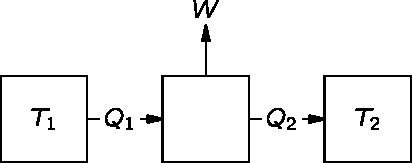
\includegraphics[width=0.8\linewidth]{fyz_fig469.pdf}
      \caption{Tepelný stroj (\cite[s.~707]{Feynman01})}
      \label{fyz:fig469}
    \end{figure}

    Carnotova analýza tepelných strojů se docela podobá argumentaci, kterou jsme používali u
    zdvižných zařízení ve kapitole \ref{fyz:IchapII} o zákonu zachování energie. Tehdy jsme vlastně
    postupovali podle Carnotova vzoru, a proto nám další úvahy budou velmi blízké.

    Předpokládejme, že jsme sestrojili tepelný stroj, jehož kotel má teplotu \(T_1\). Z kotle
    odebíráme určité teplo \(Q_1\), parní stroj vykoná určitou práci \(W\) a pára odvede určité
    teplo \(Q_2\) do chladiče s teplotou \(T_2\) (obr. \ref{fyz:fig469}). Carnot neřekl, jaké je to
    teplo, neboť neznal první zákon termodynamiky, ale ani netvrdil, že \(Q_2\) je rovno \(Q_1\),
    protože tomu nevěřil. I když ti, kteří byli ovlivnění teorií kalorika, předpokládali, že tepla
    \(Q_1\) a \(Q_2\) jsou stejná, Carnot to netvrdil a i v tom byla bystrost jeho argumentace.
    Použitím prvního termodynamického zákona bychom zjistili, že odevzdané teplo \(Q_2\) je rovno
    dodanému teplu \(Q_1\), od něhož musíme odečíst vykonanou práci \(W\):
    \begin{equation}\label{fyz:eq577}
      Q_2 = Q_1 - W
    \end{equation}
    (Kdybychom měli nějaký cyklický proces, v němž by byla zkondenzovaná voda přečerpána zpět do
    kotle, řekli bychom, že během každého cyklu bylo absorbováno teplo \(Q_1\) a vykonána práce
    \(W\) pro dané množství vody zúčastňující se cyklu.)

    Sestrojme nyní jiný stroj a zkoumej me, zda můžeme vykonat více práce při stejném dodaném teple
    při teplotě \(T_1\) a s chladičem při teplotě \(T_2\). Budeme využívat stejné množství tepla
    \(Q_1\) z kotle a pokusíme se vykonat víc práce než v případě parního stroje, třeba tak, že
    použijeme jinou kapalinu, například alkohol.

  \section{Vratné stroje}\label{fyz:IchapXLIVsecIII}
    Nyní budeme analyzovat naše stroje. Jedno je jasné, obsahuje-li stroj části, v nichž dochází ke
    tření, nevyhneme se ztrátám. Proto se uchýlíme ke stejné idealizaci jako v případě úvah o zákonu
    zachování energie - budeme předpokládat, že ve stroji vůbec nedochází ke tření.
  
    \begin{figure}[ht!] %\ref{fyz:fig470}
      \centering
      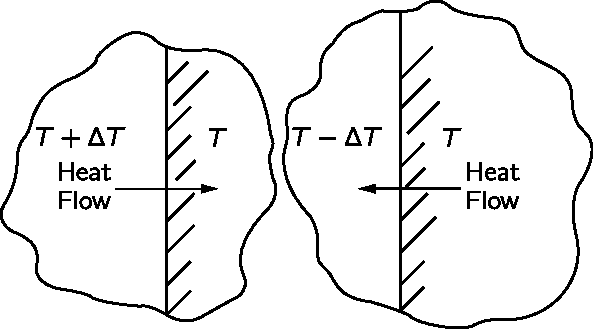
\includegraphics[width=0.9\linewidth]{fyz_fig470.pdf}
      \caption{Vratný přenos tepla (\cite[s.~707]{Feynman01})}
      \label{fyz:fig470}
    \end{figure}

    Musíme se zabývat i obdobou pohybu bez tření, kterou je tepelný přenos „bez tření“. Přiložíme-li
    horký předmět při vysoké teplotě ke studenému a vznikne tok tepla, pak není možné směr tohoto
    toku obrátit jen malou změnou teploty těchto předmětů. Máme-li však stroj bez tření a zapůsobíme
    na něj nepatrnou silou jedním směrem, bude se tím směrem pohybovat, a když na něj zapůsobíme
    nepatrnou silou v opačném směru, bude se pohybovat opačným směrem. Potřebujeme najít obdobu
    pohybu bez tření: přenos tepla, jehož směr můžeme obrátit i nepatrnou změnou. Je-li rozdíl
    teplot konečný, není to možné. Kdybychom však uskutečnili tepelný tok mezi dvěma předměty, které
    mají prakticky stejné teploty lišící se jen o infinitezimální hodnotu zabezpečující tok v
    požadovaném směru, mohli bychom mluvit o vratném toku (obr. \ref{fyz:fig470}). Zahřejeme-li
    mírně levou polovinu předmětu, poteče teplo doprava; když ji mírně ochladíme poteče teplo
    doleva. Zjistili jsme tedy, že ideálním strojem je vratný stroj, v němž je každý proces vratný v
    tom smyslu, že nepatrnými infinitezimálními změnami přinutíme stroj jít opačným směrem. Znamená
    to, že nikde ve stroji nesmí být tření ani takové místo, kde by teplo rezervoáru nebo plamene
    kotle bylo v přímém styku s něčím podstatně chladnějším nebo teplejším.

    \begin{figure}[hb!] %\ref{fyz:fig471}
      \centering
      \subcaptionbox{\label{fyz:fig471a}}{\luafigure[0.9]{fyz_fig471a.pdf}}  \newline
      \subcaptionbox{\label{fyz:fig471b}}{\luafigure[0.9]{fyz_fig471b.pdf}}  \newline
      \subcaptionbox{\label{fyz:fig471c}}{\luafigure[0.9]{fyz_fig471c.pdf}}  \newline
      \subcaptionbox{\label{fyz:fig471d}}{\luafigure[0.9]{fyz_fig471b.pdf}}
      \caption{Kroky Carnotova cyklu (\cite[s.~601]{Feynman01}).}
      \label{fyz:fig471}
    \end{figure}

    Zabývejme se nyní idealizovaným strojem, v němž jsou všechny procesy vratné. Abychom ukázali, že
    takový idealizovaný stroj je v principu možný, uvedeme příklad strojového cyklu, který může, ale
    nemusí být praktický, ale který je vratný ve smyslu Carnotovy představy. Předpokládejme, že se
    ve válci s pístem pohybujícím se bez tření nachází plyn, který nemusí být ideálním plynem.
    Nemusel by to dokonce ani být plyn, ale pro konkrétnost předpokládejme, že máme ideální plyn.
    Předpokládáme také, že máme dva tepelné polštáře, \(T_1\) a \(T_2\) - velká tělesa s určitými
    teplotami \(T_1\) a \(T_2\) (obr. \ref{fyz:fig471}). Nechť třeba \(T_1\) je vyšší než \(T_2\).
    Nejprve ohřejeme plyn za současné expanze a necháme ho ve styku s tepelným polštářem \(T_1\).
    Zatímco probíhá přívod tepla do plynu, musíme velmi pomalu zvedat píst, abychom zabezpečili, že
    teplota plynu se nikdy příliš neodchýlí od \(T_1\). Kdybychom vytahovali píst příliš rychle,
    teplota plynu by silně klesla pod \(T_1\) a proces by nebyl úplně vratný. Pohybujeme-li pístem
    dostatečně pomalu, teplota plynu se nikdy příliš neodchýlí od \(T_1\). Vrátíme-li pak píst
    pomalu zpět, teplota bude jen nepatrně vyšší než \(T_1\) a teplo poteče obráceným směrem. Je
    tedy vidět, že takové \textbf{izotermické rozpínání} (tj. probíhající při stálé teplotě), je-li
    prováděno dostatečně pomalu a jemně, je vratný proces.

    \begin{figure}[ht!] %\ref{fyz:fig472}
      \centering
      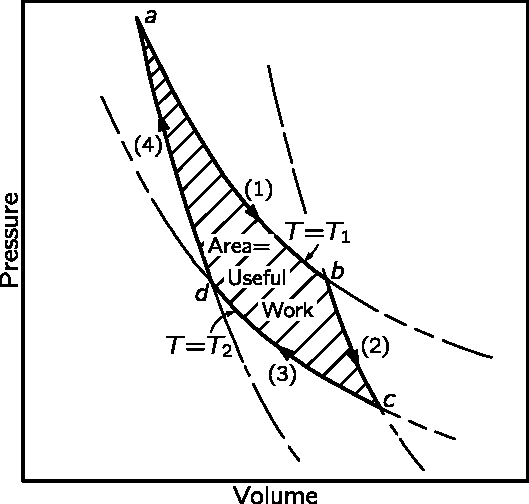
\includegraphics[width=1\linewidth]{fyz_fig472.pdf}
      \caption{Carnotův cyklus (\cite[s.~707]{Feynman01})}
      \label{fyz:fig472}
    \end{figure}

    Abychom lépe pochopili, co se děje, nakreslíme graf závislosti tlaku plynu na jeho objemu (obr.
    \ref{fyz:fig472}). Když se plyn rozpíná, tlak klesá. Křivka označená symbolem (1) nám ukazuje,
    jak se mění objem a tlak, když se teplota udržuje na hodnotě \(T_1\). V případě ideálního plynu
    by tato křivka vyjadřovala rovnici \(pV= NkT_1\). Po dobu izotermické expanze tlak se vzrůstem
    objemu klesá, dokud se nedostaneme do bodu \(b\). Současně musíme do plynu přivádět z rezervoáru
    určité teplo \(Q_1\), neboť, jak už víme, jinak by se plyn rozpínáním ochlazoval. Když jsme
    dokončili izotermickou expanzi a dostali se do bodu b, přerušíme kontakt válce s rezervoárem a
    budeme pokračovat v expanzi. Tentokrát znemožníme jakýkoliv přísun tepla k válci. Expanzi budeme
    provádět pomalu, a opět předpokládáme nepřítomnost tření, takže nebude důvod, proč bychom proces
    nemohli obrátit. Plyn pokračuje v rozpínání a teplota klesá, neboť do válce už nepřichází teplo.

    Nechme plyn rozpínat podle křivky označené (2), dokud teplota neklesne na hodnotu \(T_2\) v bodě
    označeném \(c\). Tento druh expanze bez dodání tepla se nazývá \textbf{adiabatická expanze}. Už
    víme, že v případě ideálního plynu má křivka (2) tvar \(pV^\gamma =\text{konst.}\), kde
    \(\gamma\) je konstanta větší než 1, takže adiabatická křivka má rychlejší spád než izotermická
    křivka. Plyn ve válci dosáhl teploty \(T_2\), takže když ho uvedeme do kontaktu s tepelným
    polštářem s teplotou \(T_2\), nenastanou nevratné změny. Nyní plyn pomalu stlačíme, přičemž ho
    ponecháváme ve styku s rezervoárem při teplotě  \(T_2\); toto stlačování proběhne podle křivky
    označené (3). Protože válec je ve styku s rezervoárem, teplota nevzroste, ale teplo \(Q_2\)
    proteče z válce do rezervoáru při teplotě  \(T_2\). Po izotermickém stlačení plynu podle křivky
    (3) až k bodu \(d\) odvedeme válec z tepelného polštáře s teplotou  \(T_2\) a budeme ho dále
    stlačovat, přičemž nedovolíme teplu uniknout. Teplota vzroste a tlak se bude měnit podle křivky
    označené (4). Kdybychom provedli každý krok pečlivě, vrátíme se do bodu \(a\) při teplotě
    \(T_1\), z něhož jsme vyšli a celý cyklus můžeme zopakovat znovu.

    Podle diagramu vykonal plyn úplný cyklus, v jehož průběhu jsme dodali teplo \(Q_1\) při teplotě
    \(T_1\) a odebrali teplo \(Q_2\) při teplotě \(T_2\). Důležité je, že cyklus je vratný, takže
    všechny kroky můžeme provést opačným směrem. Mohli bychom jít nazpět a ne dopředu: mohli bychom
    začít v bodě \(a\) při teplotě \(T_1\), nechat expandovat plyn podle křivky (4), dál expandovat
    při teplotě \(T_2\), absorbovat teplo \(Q_2\), atd., tedy uskutečnit Obrácený cyklus. Probíhá-li
    cyklus jedním směrem, musíme vykonat práci, probíhá-li cyklus opačně, koná práci plyn.

    Mimochodem, celkovou práci lze snadno vypočítat, protože po dobu jakékoliv expanze je práce
    rovna součinu tlaku a změny objemu, tj. \(\int p\dd{V}\). Na našem diagramu jsme vynášeli na
    svislou osu \(p\) a na vodorovnou osu \(V\). Označíme-li vertikální vzdálenost \(y\) a
    horizontální \(x\) dostaneme \(\int y\dd{x}\), tedy plochu pod křivkou. Proto plocha pod každou
    z očíslovaných křivek je mírou práce vykonané plynem nebo námi v odpovídajícím kroku. Snadno lze
    zjistit, že čistá výsledná práce je rovna obsahu vyšrafované plochy na obrázku.

    \begin{figure}[ht!] %\ref{fyz:fig473}
      \centering
      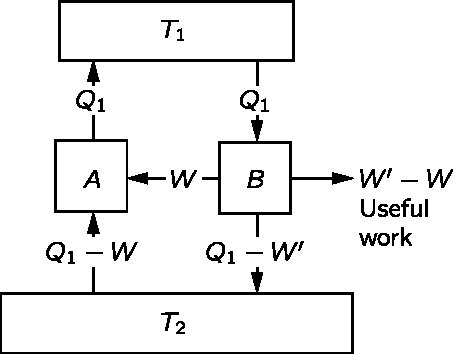
\includegraphics[width=0.8\linewidth]{fyz_fig473.pdf}
      \caption{Vratný stroj \(A\) poháněný zpětně strojem \(B\) (\cite[s.~707]{Feynman01})}
      \label{fyz:fig473}
    \end{figure}

    Nyní, když jsme ukázali jednoduchý příklad vratného stroje, budeme předpokládat, že existují i
    jiné takové stroje. Předpokládejme, že máme vratný stroj \(A\), který odebírá teplo \(Q_1\) při
    \(T_1\), koná práci \(W\) a odevzdává určité teplo při teplotě \(T_2\). Dále předpokládejme, že
    máme nějaký jiný, člověkem zkonstruovaný, stroj \(B\), už existující nebo ještě nevynalezený,
    využívající gumové pásy, páru nebo cokoliv jiného, vratný nebo nevratný, který je navržen tak,
    že odebírá stejné množství tepla \(Q_1\) při \(T_1\) a odevzdává teplo při nižší teplotě \(T_2\)
    (obr. \ref{fyz:fig473}). Předpokládejme, že stroj \(B\) koná práci \(W'\). Ukážeme, že práce \(W
    '\) není větší než \(W\) - že žádný stroj nevykonává víc práce než vratný stroj. Proč je tomu
    tak? Předpokládejme, že by \(W'\) bylo větší než \(W\). Pak můžeme vzít teplo \(Q_1\) z
    rezervoáru při teplotě \(T_1\) a pomocí stroje \(B\) konat práci \(W'\) a určité teplo odevzdat
    rezervoáru při teplotě \(T_2\): nezajímá nás, jaké teplo. Když to uděláme, můžeme ušetřit
    určitou část práce \(W'\), o níž předpokládáme, že je větší než \(W\). Odebereme jen její část
    \(W\) a zbytek \(W'-W\) využijeme k užitečné práci. S prací \(W\) necháme stroj \(A\) běžet
    opačně, protože je to \textbf{vratný stroj}. Tento stroj spotřebuje určité teplo z rezervoáru
    při \(T_2\) a odevzdá rezervoáru \(Q_1\) při \(T_1\). Při tomto dvojitém cyklu bude čistý
    výsledek takový, že se vše vrátí do původního stavu a vykonala se práce navíc, konkrétně \(W
    '-W\). Při tom vše, jsme udělali, bylo odebrání energie z rezervoáru při teplotě \(T_2\)! Teplo
    \(Q_1\) jsme pečlivě vrátili rezervoáru při teplotě \(T_1\). Proto může být rezervoár malý a
    může být uvnitř našeho složeného stroje \(A + B\), který nedělá nic jiného, než že odebírá
    množství tepla odpovídající \(W'-W\) rezervoáru při teplotě \(T_2\) a mění ho v práci. Jenže
    získání užitečné práce z rezervoáru při konstantní teplotě \emph{bez jiných změn} je podle
    Carnotova postulátu nemožné. Proto nemůže existovat stroj, který by odebíral určité množství
    tepla při vyšší teplotě \(T_1\), odevzdával jeho část při teplotě \(T_2\) a konal větší práci
    než vratný stroj pracující při stejných teplotních podmínkách.

    Nyní předpokládejme, že stroj \(B\) je také vratný. Potom, samozřejmě, nejenže \(W'\) nesmí být
    větší než \(W\), ale důkaz můžeme obrátit a ukázat, že \(W\) nemůže být větší než \(W'\).
    Jsou-li oba stroje vratné, musí konat stejnou práci a přicházíme k vynikajícímu Carnotovu
    závěru: je-li stroj vratný, nezáleží na tom, jak konkrétně je zkonstruován a práce, kterou stroj
    vykoná, absorbuje-li určité množství tepla při teplotě \(T_1\) a odevzdá určité teplo při
    teplotě \(T_2\), je \emph{u všech takových strojů stejná}. Jde o vlastnost našeho světa, a ne o
    vlastnost konkrétního stroje.

    Kdyby se nám podařilo najít zákon určující, kolik práce získáme absorbováním tepla \(Q_1\) při
    teplotě \(T_1\) a odevzdáním určitého tepla při \(T_2\) , našli bychom univerzální veličinu
    nezávislou na vlastnostech látky. Kdybychom však znali vlastnosti konkrétní látky, mohli bychom
    je využít k určení takové veličiny a pak by všechny ostatní látky musely dávat ve vratném stroji
    stejné množství práce. To je klíčová myšlenka, návod, pomocí něhož můžeme určit například
    smrštění gumy, když ji ohříváme a ochlazení gumy, když jí dovolíme smrštit se. Představme si, že
    pracovní látkou vratného stroje bude gumový pás a stroj necháme projít celým vratným cyklem.
    Čistý výsledek, celková vykonaná práce, je univerzální funkcí, úžasnou funkcí, nezávislou na
    vlastnostech látky. Tak přicházíme k přesvědčení, že existuje určité omezení vlastností látek;
    nemůžeme sestrojit, co se nám zachce, neboť jinak bychom byli schopni vymyslet látku, která by
    poskytovala víc než maximum možné práce ve vratném cyklu. Tento princip, toto omezení je jediným
    skutečným pravidlem vyplývajícím z termodynamiky.

  \section{Účinnost ideálního stroje}\label{fyz:IchapXLIVsecIV}
    Nyní se pokusíme najít zákon určující práci \(W\) jako funkci \(Q_1\), \(T_1\) a \(T_2\). Je
    jasné, že \(W\) je úměrné \(Q_1\) , neboť uvažujeme-li dva vratné stroje pracující paralelně,
    pak takový zdvojený stroj je také vratný. Absorbuje-li každý teplo \(Q_1\), pak dva spřažené
    stroje spotřebují teplo \(2Q_1\) a vykonají práci \(2W\) atd. Je proto rozumné předpokládat, že
    práce \(W\) je úměrná \(Q_1\).

    Dalším důležitým krokem bude nalezení tohoto univerzálního zákona. Budeme ho moci odvodit, když
    prozkoumáme vratný stroj s pracovní látkou, jejíž zákony známe. Takovou látkou je ideální plyn.
    K tomuto univerzálnímu zákonu bychom mohli dospět i čistě logickým uvažováním, bez použití
    nějaké konkrétní látky. Je to překrásná ukázka fyzikálního myšlení a bylo by škoda, kdybychom ji
    nemohli přednést, takže pro ty, kteří by takový důkaz rádi poznali, se o něm ještě zmíníme. Teď
    však použijeme méně abstraktní a jednodušší metodu přímého výpočtu v případě ideálního plynu.

    Potřebujeme znát pouze vztahy pro \(Q_1\) a \(Q_2\) (neboť \(W\) je \(Q_1 - Q_2\) ), tedy pro
    tepla, která si stroj vyměňuje s rezervoáry po dobu izotermického rozpínání nebo stlačování.
    Například, kolik tepla \(Q_1\) se absorbuje z rezervoáru při teplotě \(T_1\) po dobu
    izotermického rozpínání (křivka (1) na obr. \ref{fyz:fig472}) z bodu \(a\) při tlaku \(p_a\),
    objemu \(V_a\), teplotě \(T_1\) do bodu \(b\) s tlakem \(p_b\), objemem \(V_b\) a stejnou
    teplotou \(T_1\)? V případě ideálního plynu má každá molekula energii, jež závisí jen na
    teplotě, a protože jsou teplota i počet molekul stejné v \(a\) i \(b\), bude vnitřní energie
    stejná. \emph{Energie \(U\) se nemění}; práce, kterou koná plyn po dobu expanze 
    \begin{equation*}
      W=∫^b_ap\dd{V},
    \end{equation*}
    je rovna energii \(Q_1\) odebrané z rezervoáru. Po dobu rozpínání \(pV= NkT_1\), neboli
    \begin{equation}\label{fyz:eq671}
      p=\frac{NkT_1}{V}
    \end{equation}
    nebo
    \begin{equation}\label{fyz:eq672}
      Q_1=∫^b_ap\dd{V}=∫^b_aNkT_1\frac{\dd{V}}{V}
    \end{equation}
    nebo
    \begin{equation}\label{fyz:eq673}
      Q_1=NkT_1\ln\frac{V_b}{V_a}.
    \end{equation}
    Tento výraz představuje teplo odebrané z rezervoáru při teplotě \(T_1\). Stejným způsobem můžeme
    určit teplo odevzdané při teplotě \(T_2\) (křivka (3) obr. \ref{fyz:fig472}) rezervoáru po dobu
    stlačování. Tak dostaneme
    \begin{equation}\label{fyz:eq674}
      Q_2=NkT_2\ln\frac{V_c}{V_d}.
    \end{equation}
    K ukončení našeho rozboru potřebujeme ještě najít vztah mezi \(V_c/V_d\) a \(V_b/V_a\). Tento
    vztah najdeme, když si uvědomíme, že (2) představuje adiabatické rozpínání z \(b\) do \(c\), po
    dobu kterého je \(pV^\gamma\) konstantní. Když \(pV= NkT\), můžeme psát \((pV)\cdot V^{\gamma
    -1} = \text{konst}\) nebo to vyjádřit pomocí \(T\) a \(V\) ve tvaru \(TV^{\gamma - 1} =
    \text{konst.}\), tedy
    \begin{equation}\label{fyz:eq675}
      T_1V^{γ−1}_b=T_2V^{γ−1}_c.
    \end{equation}
    Podobně (4) také představuje adiabatické rozpínání, a to z \(d\) do \(a\), takže můžeme psát
    \begin{equation}\label{fyz:eq676}
      T_1V^{γ−1}_a=T_2V^{γ−1}_d.
    \end{equation}
    Vydělíme-li tuto rovnici předcházející, dostaneme rovnost výrazů \(V_b/V_a\) a \(V_c/V_d\).
    Proto logaritmy v (\ref{fyz:eq673}) a (\ref{fyz:eq673}) musí být stejné a máme
    \begin{equation}\label{fyz:eq677}
      \frac{Q_1}{T_1}=\frac{Q_2}{T_2}.
    \end{equation}
    To je vztah, který jsme hledali. I když jsme ho dokázali pouze pro stroj pracující s ideálním
    plynem, musí být správný \emph{pro jakýkoliv matný stroj}.

    \begin{figure}[ht!] %\ref{fyz:fig474}
      \centering
      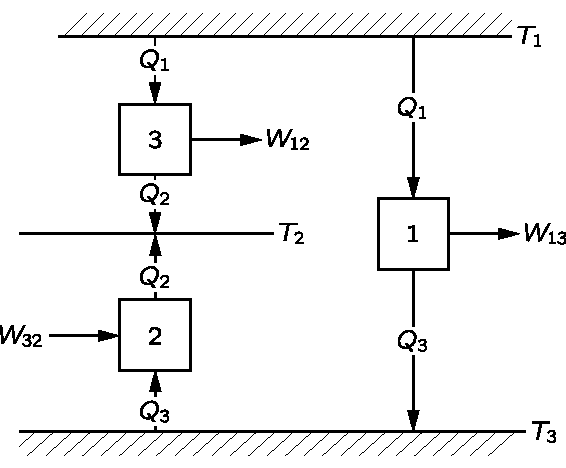
\includegraphics[width=0.9\linewidth]{fyz_fig474.pdf}
      \caption{Spojení strojů 1 a 2 je ekvivalentní stroji 3 (\cite[s.~707]{Feynman01})}
      \label{fyz:fig474}
    \end{figure}

    Nyní ukážeme, jak můžeme k tomuto univerzálnímu zákonu dospět logickou cestou bez znalosti
    vlastností nějaké konkrétní látky. Předpokládejme, že máme tři stroje a tři teploty, např.
    \(T_1\), \(T_2\) a \(T_3\). Nechť jeden stroj absorbuje teplo \(Q_1\) při teplotě \(T_1\),
    vykoná určité množství práce \(W_{13}\) a odevzdá teplo \(Q_3\) při teplotě \(T_3\) (obr.
    \ref{fyz:fig474}). Nechť druhý stroj pracuje opačným způsobem mezi teplotami \(T_2\) a \(T_3\).
    Předpokládejme, že tento druhý stroj je tak velký, že absorbuje právě teplo \(Q_3\) a odevzdá
    teplo \(Q_2\). Musíme na něj vynaložit určité množství práce \(W_{32}\) - tato práce bude
    záporná, neboť stroj pracuje v obráceném cyklu. Když první stroj ukončí cyklus, absorbuje teplo
    \(Q_1\) a odevzdá teplo \(Q_3\) při teplotě \(T_3\); druhý stroj odebere stejné teplo \(Q_3\)
    při teplotě \(T_3\); z rezervoáru a odevzdá ho rezervoáru při teplotě \(T_2\). Proto čistý
    výsledek takových spřažených strojů je odebrání tepla \(Q_1\) při teplotě \(T_1\) a odevzdání
    tepla \(Q_2\) při teplotě \(T_2\). Tyto dva stroje jsou proto ekvivalentní třetímu, který
    absorbuje \(Q_1\) při teplotě \(T_1\), koná práci \(W_{12}\) a odevzdává teplo \(Q_2\) při
    \(T_2\). Přitom \(W_{12} = W_{13} – W_{32}\), jak vyplývá z prvního zákona
    \begin{align}
      W_{13}−W_{32}&=(Q_1-Q_3)-(Q_2-Q_3) \nonumber \\
                   &=Q_1-Q_2=W_{12}.     \label{fyz:eq678}
    \end{align}
    Nyní můžeme získat zákony dávající do vzájemného vztahu účinnosti strojů; vždyť je jasné, že
    musí existovat určitý druh závislosti mezi účinnostmi strojů pracujících mezi teplotami \(T_1\)
    a \(T_3\), mezi \(T_2\) a \(T_3\) a mezi \(T_1\) a \(T_2\).

    Naše argumenty budou velmi jasné, budeme-li postupovat následujícím způsobem: Zjistili jsme, že
    teplo absorbované při \(T_1\) můžeme vždy dát do souvislosti s teplem odevzdaným při \(T_2\),
    určíme-li teplo odevzdané při nějaké jiné teplotě \(T_3\). Proto budeme moci popsat všechny
    vlastnosti stroje, zavedeme-li určitou standardní teplotu a naši analýzu provedeme právě při
    této standardní teplotě. Jinak řečeno, známe-li účinnost stroje pracujícího mezi určitou
    teplotou \(T\) a jakousi standardní teplotou, budeme moci vypočítat účinnost pro jakýkoliv jiný
    rozdíl teplot. Protože předpokládáme pouze použití vratných strojů můžeme přejít od počáteční
    teploty dolů ke standardní teplotě a pak přejít zpět k výsledné teplotě. Standardní teplotu
    můžeme vybrat libovolně a zvolíme za ni \emph{jeden stupeň}. Pro teplo, jež se odevzdává při
    této standardní teplotě, zavedeme zvláštní symbol \(Q_S\). Jinými slovy: absorbuje-li vratný
    stroj při teplotě \(T\) teplo \(Q\), pak při jednotkové teplotě odevzdá teplo \(Q_S\).
    \emph{Odevzdá-li nějaký stroj absorbující teplo \(Q_S\) při teplotě \(T_1\) teplo \(Q_1\) při
    teplotě jednoho stupně a odevzdá-li druhý stroj absorbující teplo \(Q_2\) při teplotě \(T_2\)
    také teplo \(Q_S\) při teplotě jednoho stupně, pak podle našeho důkazu týkajícího se strojů
    pracujících mezi třemi teplotami musí stroj, který absorbuje teplo \(Q_1\) při teplotě \(T_1\),
    odevzdat teplo \(Q_2\), pracuje-li mezi teplotami \(T_1\) a \(T_2\)}. Už nám zbývá jen najít,
    kolik tepla \(Q_S\) musíme dodat při teplotě \(T_1\), abychom odevzdali určité množství tepla
    \(Q_1\) při jednotkové teplotě. Jakmile to zjistíme, máme vyhráno. Samozřejmě teplo \(Q\) je
    funkcí teploty \(T\). Snadno se zjistí, že se vzrůstem teploty musí vzrůstati teplo, protože
    víme, že na zpětný chod stroje a odevzdání tepla při vyšší teplotě se spotřebuje práce. Není
    těžké pochopit, že teplo \(Q_1\) musí být úměrné \(Q_S\). Potom náš velký zákon musí vypadat
    takto: Danému množství tepla \(Q_S\) odevzdanému při jednom stupni odpovídá množství tepla \(Q\)
    absorbované strojem při teplotě \(T\) a toto množství je rovno součinu \(Q_S\) a určité rostoucí
    funkce teploty:
    \begin{equation}\label{fyz:eq679}
      Q=Q_Sf(T).
    \end{equation}

  \section{Termodynamická teplota}\label{fyz:IchapXLIVsecV}
    Zatím se nepokusíme najít vztah pro zmíněnou rostoucí funkci teploty vyjádřenou pomocí stupnice
    známého rtuťového teploměru, ale místo toho \emph{definujeme novou teplotní stupnicí}. Kdysi byla
    „teplota“ definována libovolně rozdělením objemu vody roztahující se teplem na stejné stupně
    určité velikosti. Když se však teplota měřila rtuťovým teploměrem, zjistilo se, že stupňům už
    neodpovídají stejné vzdálenosti na stupnici. Nyní \emph{však můžeme definovat teplotu, která
    nezávisí na vlastnostech látky}. Můžeme k tomu využít uvedenou funkci \(f(T)\), která nezávisí
    na použitém zařízení, protože účinnost vratných strojů nezávisí na jejich pracovních látkách.
    Protože tato funkce s růstem teploty roste, můžeme ji \emph{samotnou} považovat za teplotu
    měřenou v standardních jednotkách takto:
    \begin{equation}\label{fyz:eq691}
      Q=ST,
    \end{equation}
    kde
    \begin{equation}\label{fyz:eq692}
      Q_S=S\cdot\SI{1}{\celsius},
    \end{equation}

    \begin{figure}[ht!] %\ref{fyz:fig475}
      \centering
      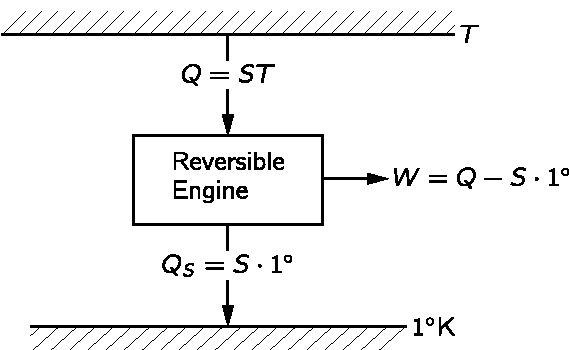
\includegraphics[width=0.9\linewidth]{fyz_fig475.pdf}
      \caption{Absolutní termodynamická teplota (\cite[s.~707]{Feynman01})}
      \label{fyz:fig475}
    \end{figure}

    To znamená, že teplotu tělesa určíme tak, že zjistíme, kolik tepla absorboval vratný stroj
    pracující mezi teplotou tělesa a jednotkovou teplotou (obr. \ref{fyz:fig475}). Když se z kotle
    odebere sedmkrát víc tepla, než se odevzdá jednostupňovému chladiči, říkáme, že tento kotel má
    teplotu sedm stupňů atd. \footnote{Termodynamickou teplotu dnes udáváme v jednotkách zvaných
    kelvin} Měřením množství tepla absorbovaného při různých teplotách určujeme teplotu. Takto
    definovanou teplotu nazýváme \textbf{absolutní termodynamickou teplotou} a tato teplota nezávisí
    na pracovní látce. Dále budeme výlučně používat tuto definici teploty\footnote{Předtím jsme naši
    teplotní stupnici definovali jiným způsobem, konkrétně tak, že jsme střední kinetickou energii
    molekuly ideálního plynu považovali za úměrou teplotě, tedy ve shodě se zákonem ideálního plynu
    jsme považovali \(pV\) úměrně \(T\). Je taková definice ekvivalentní naší nové definici? Na tuto
    otázku můžeme odpovědět kladně, neboť konečný výsledek (\ref{fyz:eq677}), odvozený ze zákona
    ideálního plynu, je stejný jako zde odvozený výsledek. V další kapitole se ještě k tomuto
    problému vrátíme.}.

    Nyní je nám jasné, že v případě dvou strojů, z nichž jeden pracuje mezi \(T_1\) a jedním stupněm
    druhý mezi \(T_2\) a jedním stupněm a oba odevzdávají stejné teplo při jednotkové teplotě, musí
    pro absorbovaná tepla platit vztah
    \begin{equation}\label{fyz:eq701}
      \frac{Q_1}{T_1} = S = \frac{Q_2}{T_2}. 
    \end{equation}
    Kdybychom tedy měli jednoduchý stroj pracující mezi \(T_1\) a \(T_2\), pak by výsledek naší
    analýzy, to velké finále, spočíval v tom, že poměr \(Q_1/T_1\) je stejný jako poměr \(Q_2/T_2\),
    absorbuje-li stroj energii \(Q_1\) při teplotě \(T_1\) a odevzdá teplo \(Q_2\) při teplotě
    \(T_2\). Tento vztah musí platit pro libovolný vratný stroj. K tomu je třeba dodat už jen tolik,
    že jde o nejdůležitější výrok celé termodynamiky.

    Představuje-li však toto vlastně celou termodynamiku, proč bývá považována za náročný předmět?
    Máte-li danou hmotnost látky, můžete stav této látky v kterémkoliv okamžiku popsat udáním její
    teploty a objemu. Známe-li teplotu a objem látky a víme, že tlak je určitou funkcí teploty a
    objemu, budeme znát vnitřní energii. jenže někdo si řekne: \uv{Já to tak nebudu dělat! Řekněte
    mi, jaká je teplota a jaký je tlak a já vám řeknu, jaký je objem. objem můžu považovat za funkci
    teploty a tlaku a vnitřní energii za funkci teploty a tlaku atd.} Příčina náročnosti
    termodynamiky spočívá právě v tom, že každý používá jiný přístup. Kdybychom se však uměli
    dohodnout na našich proměnných a tuto dohodu i dodržovali, termodynamika by byla docela snadná.

    Nyní se pustíme do dedukování. Tak jako \(F = ma\) představovalo ústřední rovnici celé mechaniky
    a vše jsme z ní odvozovali, bude právě nalezený princip představovat základ celé termodynamiky.
    A my se ptáme, jaké závěry z něho můžeme udělat.

    Abychom mohli udělat první závěr, zkombinujeme oba zákony - zákon zachování energie a zákon
    dávající do souvislosti tepla \(Q_2\) a \(Q_1\) a dospějeme k \emph{účinností vratného stroje}.
    Z prvního zákona máme \(W= Q_1 – Q_2\). Podle našeho nového principu
    \begin{equation*}
      Q_2=\frac{T_2}{T_1}Q_1,
    \end{equation*}
    a pro práci dostáváme vztah
    \begin{equation}\label{fyz:eq702}
      W=Q_1\left(1−\frac{T_2}{T_1}\right)=Q_1\frac{T_1−T_2}{T_1},
    \end{equation}   
    který určuje účinnost stroje - říká, kolik práce získáme z určitého množství tepla. Účinnost
    stroje je úměrná rozdílu teplot, mezi nimiž stroj pracuje, dělenému vyšší teplotou
    \begin{equation}\label{fyz:eq703}
      \text{účinnost} = \frac{W}{Q_1}=\frac{T_1−T_2}{T_1}.
    \end{equation} 
    Účinnost nemůže být větší než jedna a absolutní teplota nemůže být menší než nula, absolutní
    nula. Protože \(T_2\) musí být kladné, účinnost je vždy menší než jedna. To je náš první
    výsledek.

  \section{Entropie}\label{fyz:IchapXLIVsecVI}
    Rovnici (\ref{fyz:eq677}) nebo (\ref{fyz:eq701}) můžeme interpretovat zvláštním způsobem.
    Pracujeme-li s vratnými stroji, je teplo \(Q_1\) při teplotě \(T_1\) „ekvivalentní“ \(Q_2\) při
    \(T_2\) neboli \(\frac{Q_1}{ T_1} = \frac{Q_2}{T_2}\) v tom smyslu, že je-li jedno z tepel
    absorbováno, je druhé odevzdáno. Kdybychom tedy nějak nazvali veličinu \(\frac{Q}{T}\), mohli
    bychom prohlásit: ve vratných procesech je absorbováno tolik \(\frac{Q}{T}\), kolik je uvolněno;
    \(\frac{Q}{T}\) se ani nezískává, ani neztrácí. Poměr \(\frac{Q}{T}\) nazýváme \textbf{entropie}
    a říkáme, že „ve vratném cyklu je změna entropie nulová“. Když \(T\) je \SI{1}{\celsius}, pak je
    entropie \(\frac{Q}{\SI{1}{\celsius}}\), nebo, jak jsme již označili,
    \(\frac{Q}{\SI{1}{\celsius}} = S\). Opravdu \(S\) je písmeno, které nejčastěji používáme pro
    entropii a ta je číselně rovna teplu (které jsme označili \(Q_S\)) dodanému rezervoáru při
    jednotkové teplotě (samotná entropie není teplo, ale představuje teplo dělené teplotou a měří se
    v joulech na stupeň)\footnote{joulech na kelvin}.
    
    Je zajímavé, že kromě tlaku, který je funkcí teploty, objemu a vnitřní energie, jež je také
    funkcí teploty a objemu, jsme našli jinou veličinu, která je funkcí stavu a tou je entropie
    látky. Pokusme se vysvětlit, jak se tato veličina počítá a co rozumíme tím, když říkáme, že je
    „funkcí stavu“. Uvažujme systém ve dvou různých stavech, například takových, jaké jsme měli v
    experimentu s adiabatickou a izotermickou expanzí. (Mimochodem, stroj nemusí mít nezbytně dva
    rezervoáry; můžou být tři nebo čtyři různé teploty, při nichž odebírá a odevzdává teplo.) Můžeme
    se pohybovat po celém \(pV\)-diagramu a přecházet z jednoho stavu do druhého. Jinak řečeno, plyn
    můžeme převádět z určitého stavu \(a\) do jiného stavu \(b\) a přitom požadovat, aby tento
    přechod z \(a\) do \(b\) byl vratný. Nyní předpokládejme, že podél dráhy z \(a\) do \(b\) máme
    malé rezervoáry s různými teplotami, takže teplo odebrané látce při každém drobném kroku je
    odevzdáno každému rezervoáru při teplotě odpovídající příslušnému bodu dráhy. Pak připojme
    všechny tyto rezervoáry vratnými tepelnými stroji k jednomu rezervoáru při jednotkové teplotě.
    Když ukončíme převod látky z \(a\) do \(b\), vraťme všechny rezervoáry do jejich původního
    stavu. Každé teplo \(\dif Q\), které bylo odebráno látce při teplotě \(T\), jsme takto přeměnili
    vratným strojem a při jednotkové teplotě bylo odevzdáno určité množství entropie \(\dif S\),
    jmenovitě
    \begin{equation}\label{fyz:eq704}
      \dif S=\frac{\dif Q}{T}.
    \end{equation}

    Vypočítejme celkové množství odevzdané entropie. Rozdíl entropií neboli entropie potřebná k
    přechodu z \(a\) do \(b\) při takové vratné transformaci představuje celkovou entropii -
    celkovou entropii odebranou z malých rezervoárů a odevzdanou při jednotkové teplotě:
    \begin{equation}\label{fyz:eq705}
      S_b−S_a=∫^b_a\frac{\dif Q}{T}.
    \end{equation}

    \begin{figure}[ht!] %\ref{fyz:fig476}
      \centering
      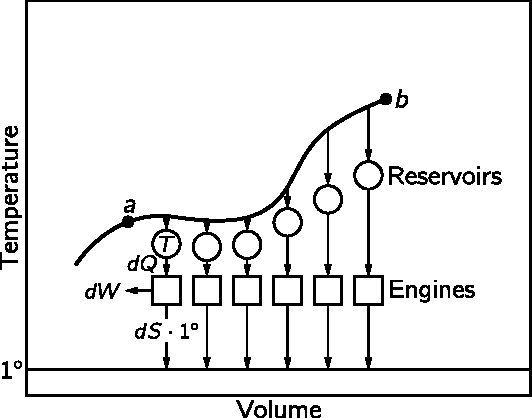
\includegraphics[width=0.9\linewidth]{fyz_fig476.pdf}
      \caption{Změna entropie při vratném přechodu (\cite[s.~707]{Feynman01})}
      \label{fyz:fig476}
    \end{figure}

    Nyní se ptáme, zda rozdíl entropií závisí na zvolené dráze. Existuje totiž víc způsobů, jak se
    dostat z \(a\) do \(b\). Vzpomeňme si, že při Carnotově cyklu jsme podle obr. \ref{fyz:fig472}
    mohli přejít z \(a\) do \(c\) nejprve izotermickou expanzí a pak adiabaticky nebo nejprve
    adiabatickou expanzí a pak izotermicky. Zajímá nás proto, zda je změna entropie, která nastává,
    když přecházíme z \(a\) do \(b\) podle obr. \ref{fyz:fig476}, pro každou dráhu stejná. Musí být
    stejná, neboť kdybychom završili celý cyklus jednou dráhou tam a druhou zpět, měli bychom vratný
    stroj a nemohly by nastat ztráty tepla do rezervoáru při jednotkové teplotě. Ve zcela vratném
    cyklu nesmí být odebráno žádné teplo z rezervoáru při jednotkové teplotě, a tak je entropie
    potřebná k přechodu z \(a\) do \(b\) pro kteroukoliv dráhu stejná. \emph{Nezávisí na samotné
    dráze}, závisí jen na koncových bodech. Proto můžeme tvrdit, že existuje určitá funkce, kterou
    nazýváme entropie látky a která závisí pouze na stavu, tj. jen na objemu a teplotě.

    Můžeme najít funkci \(S(V,T)\), jež má tu vlastnost, že při vratných změnách látky má změna
    entropie vyjádřená pomocí tepla odevzdaného při jednotkové teplotě následující tvar
    \begin{equation}\label{fyz:eq706}
      ΔS=∫\frac{\dif Q}{T},
    \end{equation}
    kde \(\dif Q\) teplo odebrané látce při teplotě \(T\). Tato celková změna entropie je rozdíl
    entropie vypočítané v koncovém a počátečním bodě dráhy
    \begin{equation}\label{fyz:eq707}
      ΔS=S(V_b,T_b)−S(V_a,T_a)=∫^b_a\frac{\dif Q}{T}.
    \end{equation}
    Tento výraz nedefinuje entropii úplně. Definuje vlastně jen rozdíl entropie ve dvou různých
    stavech. Jen tehdy, když umíme vypočítat entropii jednoho konkrétního stavu, můžeme definovat
    entropii \(S\) absolutně.

    Dlouho se předpokládalo, že absolutní entropie neznamená nic a že je možné definovat pouze
    rozdíly entropie. Nakonec však přišel Nernst s velmi jednoduchým tvrzením, které nazval „věta o
    teple“ a kterému dnes říkáme \textbf{třetí zákon termodynamiky}. Povíme si, co tento zákon říká,
    ale nebudeme vysvětlovat, proč platí. Nernstův postulát prostě tvrdí, že každý objekt má při
    absolutní nule nulovou entropii. Nyní už víme, při kterém \(T\) a \(V\) je \(S\) nulové
    (konkrétně při \(T=0\)), a proto můžeme entropii určit v libovolném jiném bodě.

    \begin{figure}[ht!] %\ref{fyz:fig477}
      \centering
      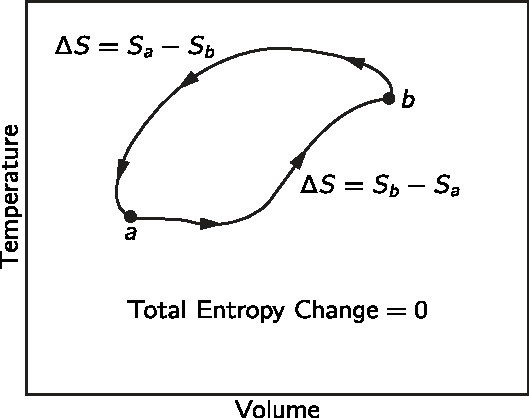
\includegraphics[width=0.9\linewidth]{fyz_fig477.pdf}
      \caption{Změna entropie při úplném vratném cyklu (\cite[s.~707]{Feynman01})}
      \label{fyz:fig477}
    \end{figure}

    Abychom ilustrovali tyto myšlenky, vypočítejme entropii ideálního plynu. Při izotermické (a tedy
    i vratné) expanzi je \(∫\dif Q/T\) rovno \(\frac{Q}{T}\), protože \(T\) je konstanta. Proto (v
    souhlase se vztahem \ref {fyz:eq673}) platí pro změnu entropie
    \begin{equation*}
      S(V_a,T)−S(V_b,T)=Nk\ln\frac{V_a}{V_b},
    \end{equation*}
    takže \(S(V, T) = Nk\ln V\) plus nějaká funkce jen teploty \(T\). Jak S závisí na \(T\)? Víme,
    že v případě vratné adiabatické expanze \emph{nedochází k výměně tepla}. Proto se entropie
    nemění, i když se mění \(V\), ale aby platilo \( TV^{γ−1}=\text{konst}\), musí se měnit i
    teplota \(T\). Chápeme, že musí být
    \begin{equation*}
      S(V,T)=Nk\left[\ln V + \frac{1}{γ−1}\ln T\right] + a,
    \end{equation*}
    kde \(a\) je nějaká konstanta, která nezávisí na \(V\), ani na \(T\)? (Konstanta \(a\) se nazývá
    chemická konstanta. Závisí na zkoumaném plynu a můžeme ji experimentálně určit z Nernstovy věty
    měřením tepla uvolňovaného při ochlazování a kondenzaci plynu až po jeho přeměnu na tuhou látku
    (v případě hélia kapalnou) při nulové teplotě; přitom je třeba vypočítat integrál \(∫\frac{\dif
    Q}{T}\). Konstantu \(a\) můžeme určit i teoreticky pomocí Planckovy konstanty a kvantové
    mechaniky, ale v tomto kurzu se tím nebudeme zabývat.)

    Nyní si všimněme některých vlastností entropie. Vzpomeňme si, že na úseku vratného cyklu od
    \(a\) do \(b\) se entropie látky mění o \(S_b – S_a\). Dále si vzpomeňme, že při takovém
    postupu entropie - teplo odevzdané při jednotkové teplotě - vzrůstá podle Zákona \(\dif S =
    \frac{\dif Q}{T}\), kde \(\dif Q\) je teplo, které odebereme látce při teplotě \(T\).

    Už víme, že při vratném cyklu se celková entropie všeho nemění, neboť teplo \(Q_1\) absorbované
    při \(T_1\) a teplo \(Q_2\) odevzdané při \(T_2\) odpovídají stejně velkým, ale opačným změnám
    entropie, takže výsledná změna entropie je nulová. Proto se při vratném cyklu nemění entropie
    žádné části, ani rezervoárů. Toto pravidlo se podobá zákonu zachování energie, ale tím není;
    platí totiž pouze pro vratné cykly. Kdybychom uvažovali i nevratné cykly, žádný zákon zachování
    entropie neplatí.

    Uvedeme dva příklady. Nejprve předpokládáme, že nevratnou práci koná objekt, v němž existuje
    tření a který produkuje teplo \(Q\) při teplotě \(T\). Entropie vzroste o \(\frac{Q}{T}\). Teplo
    \(Q\) je rovno práci, a proto, když konáme nějakou práci třením předmětu, jehož teplota je
    \(T\), vzrůstá entropie o \(\frac{W}{T}\).

    Další příklad nevratnosti spočívá v následujícím: Spojíme-li dva předměty s různými teplotami
    \(T_1\) a \(T_2\), přejde určité množství tepla samovolně z jednoho předmětu na druhý. Například
    předpokládejme, že jsme do studené vody vložili horký kámen. Jak se změní entropie horkého
    kamene, když odevzdá teplo \( ΔQ\) z \(T_1\) na \(T_2\)? Poklesne o \(\frac{ΔQ}{T_1}\). Jak se
    změní entropie vody? Vzroste o \(\frac{ΔQ}{T_2}\). Teplo však poteče jen od vyšší teploty
    \(T_1\) k nižší teplotě \(T_2\), takže \( ΔQ\)  je kladné, je-li teplota \(T_1\) je vyšší než
    teplota \(T_2\). Proto je změna entropie celého světa kladná a je rovna se rozdílu dvou zlomků
    \begin{equation}\label{fyz:eq708}
      ΔS=\frac{ΔQ}{T_2}−\frac{ΔQ}{T_1}.
    \end{equation}

    Platí tedy toto tvrzení: V každém nevratném procesu entropie všeho na světě vzrůstá.]en ve
    vratných procesech zůstává entropie konstantní. Protože však žádný proces není absolutně vratný,
    entropie vždy aspoň o málo vzroste; vratný proces je idealizace s minimálním přírůstkem
    entropie.

    Bohužel, v termodynamice nepůjdeme do hloubky. Naším cílem je jen ilustrace základních
    myšlenek a vysvětlení používané argumentace, ale termodynamikou se příliš zabývat nebudeme.
    Termodynamiku velmi často používají technici a hlavně chemici, proto musíme učit termodynamiku v
    chemické nebo technické praxi. Není vhodné všechno opakovat, omezujeme se pouze na diskuzi o
    povaze této teorie a nevěnujeme se detailům speciálních aplikací.

    Dva zákony termodynamiky jsou často formulovány takto:
    \begin{itemize}[noitemsep]
      \item \emph{První zákon}: energie vesmíru je vždy konstantní.
      \item \emph{Druhý zákon}: entropie vesmíru vždy vzrůstá.
    \end{itemize}

    Formulace druhého zákona není právě nejvhodnější, protože například nevyjadřuje, že ve vratném
    cyklu se entropie nemění a přesně neříká, co vlastně entropie je. Je to jen způsob vhodný k
    zapamatování těchto zákonů, ale ve skutečnosti nám přesně neříká, na čem jsme. Zákony
    diskutované v této kapitole jsou shrnuty v tabulce 44.1. V další kapitole využijeme tyto zákony
    k získání vztahu mezi teplem generovaným při rozpínání pásku gumy a dodatečným vnitřním napětím
    při jeho zahřívání.

    \begin{mdframed}[style=mdnote]
      \begin{note}Shrnutí termodynamických zákonů:
        \begin{itemize}[noitemsep]
          \item \textbf{První zákon}: teplo dodané systému + práce konaná na systému = vzrůst
                vnitřní energie systému 
                \begin{equation*}
                  \dif Q + \dif W=\dif U.
                \end{equation*}
          \item \textbf{Druhý zákon}: Proces, jehož jediným čistým výsledkem by bylo odebrání tepla
                z rezervoáru a jeho přeměna na práci je nemožná. Žádný tepelný stroj odebírající
                teplo \(Q_1\) při \(T_1\) a odevzdávající teplo \(Q_2\) při \(T_2\) nemůže vykonat
                víc práce než vratný stroj, pro nějž platí
                \begin{equation*}
                  W=Q_1−Q_2=Q_1\left(\frac{T_1−T_2}{T_1}\right).
                \end{equation*}
          \item \textbf{Definice entropie systému}:
                \begin{itemize}
                  \item je-li teplo \( ΔQ\) vratně dodáno systému při teplotě \(T\), vzroste
                        entropie systému o \(ΔS=\frac{ΔQ}{T}\)
                  \item Při \(T=0\), \(S=0\) (třetí zákon).
                \end{itemize}  
                Při \emph{vratně změně} se celková entropie všech částí systému (včetně rezervoárů)
                nemění.
                
                Při \emph{nevratné změně} celková entropie systému vždy vzrůstá.  
        \end{itemize}
      \end{note}
    \end{mdframed}
  
  \section{Příklady a cvičení}\label{fyz:IchapXLIVsecVII}
%---------------------------------------------------------------------------------------------------